%%%%%%%%%%%%%%%%%%%%%%%%%%%%% Define Article %%%%%%%%%%%%%%%%%%%%%%%%%%%%%%%%%%
\documentclass[10pt,a4paper,openany]{article}

%%%%%%%%%%%%%%%%%%%%%%%%%%%%%%%%%%%%%%%%%%%%%%%%%%%%%%%%%%%%%%%%%%%%%%%%%%%%%%%
\usepackage[utf8]{inputenc}
\usepackage[T1]{fontenc}
%%%%%%%%%%%%%%%%%%%%%%%%%%%%% Using Packages %%%%%%%%%%%%%%%%%%%%%%%%%%%%%%%%%%
\usepackage{graphicx}
\usepackage{amssymb}
\usepackage{amsmath}
\usepackage{amsthm}
\usepackage{empheq}
\usepackage{mdframed}
\usepackage{booktabs}
\usepackage{lipsum}
\usepackage{ifthen}
\usepackage{graphicx}
\usepackage{color}
\usepackage{psfrag}
\usepackage{pgfplots}
\usepackage{bm}
%%%%%%%%%%%%%%%%%%%%%%%%%%%%%%%%%%%%%%%%%%%%%%%%%%%%%%%%%%%%%%%%%%%%%%%%%%%%%%%
\usepackage[colorlinks=true]{hyperref}
\hypersetup{
    colorlinks=true,
    linkcolor=blue!50!black,
    filecolor=blue!50!black,
    citecolor = green!50!black,      
    urlcolor=cyan,
}
\usepackage{mathtools}
\usepackage{amsthm}
\usepackage{empheq}
\usepackage{bm}
\usepackage{tikz}
\usepackage{subcaption}
\usepackage{multicol}
\usepackage[left=1.5cm,right=1.5cm,top=2cm,bottom=2cm]{geometry}
% Other Settings
\usepackage{wasysym}
\usepackage{ifthen}

%%%%%%%%%%%%%%%%%%%%%%%%%% Page Setting %%%%%%%%%%%%%%%%%%%%%%%%%%%%%%%%%%%%%%%

\usepackage{natbib}
\bibliographystyle{apalike}

\usepackage{enumitem}
\setlist{nolistsep}
%%%%%%%%%%%%%%%%%%%%%%%%%% Define some useful colors %%%%%%%%%%%%%%%%%%%%%%%%%%
\definecolor{ocre}{RGB}{243,102,25}
\definecolor{mygray}{RGB}{243,243,244}
\definecolor{deepGreen}{RGB}{26,111,0}
\definecolor{shallowGreen}{RGB}{235,255,255}
\definecolor{deepBlue}{RGB}{61,124,222}
\definecolor{shallowBlue}{RGB}{235,249,255}
\definecolor{vertcanard}{RGB}{0,69,78}
\definecolor{darkred}{RGB}{84,10,0}
\definecolor{saumon}{RGB}{100,49,42}
%%%%%%%%%%%%%%%%%%%%%%%%%%%%%%%%%%%%%%%%%%%%%%%%%%%%%%%%%%%%%%%%%%%%%%%%%%%%%%%

%%%%%%%%%%%%%%%%%%%%%%%%%% Define an orangebox command %%%%%%%%%%%%%%%%%%%%%%%%
\newcommand\orangebox[1]{\fcolorbox{ocre}{mygray}{\hspace{1em}#1\hspace{1em}}}
%%%%%%%%%%%%%%%%%%%%%%%%%%%%%%%%%%%%%%%%%%%%%%%%%%%%%%%%%%%%%%%%%%%%%%%%%%%%%%%

%%%%%%%%%%%%%%%%%%%%%%%%%%%% English Environments %%%%%%%%%%%%%%%%%%%%%%%%%%%%%
\newtheoremstyle{mytheoremstyle}{3pt}{3pt}{\normalfont}{0cm}{\rmfamily\bfseries}{}{1em}{{\color{black}\thmname{#1}~\thmnumber{#2}}\thmnote{\,--\,#3}}
\newtheoremstyle{myproblemstyle}{3pt}{3pt}{\normalfont}{0cm}{\rmfamily\bfseries}{}{1em}{{\color{black}\thmname{#1}~\thmnumber{#2}}\thmnote{\,--\,#3}}
\theoremstyle{mytheoremstyle}
\newmdtheoremenv[linewidth=1pt,backgroundcolor=shallowGreen,linecolor=deepGreen,leftmargin=0pt,innerleftmargin=20pt,innerrightmargin=20pt,]{theorem}{Theorem}[section]
\theoremstyle{mytheoremstyle}
\newmdtheoremenv[linewidth=1pt,backgroundcolor=shallowBlue,linecolor=deepBlue,leftmargin=0pt,innerleftmargin=20pt,innerrightmargin=20pt,]{definition}{Definition}[section]
\theoremstyle{myproblemstyle}
\newmdtheoremenv[linecolor=black,leftmargin=0pt,innerleftmargin=10pt,innerrightmargin=10pt,]{problem}{Problem}[section]
%%%%%%%%%%%%%%%%%%%%%%%%%%%%%%%%%%%%%%%%%%%%%%%%%%%%%%%%%%%%%%%%%%%%%%%%%%%%%%%
\usepackage{fancyhdr}
\renewcommand{\figurename}{\color{orange!90!black}{\textsc{Figure.}}}%
\renewcommand{\tablename}{\color{orange!90!black}{\textsc{Table.}}}%
\AtBeginDocument{\renewcommand{\ref}[1]{\autoref{#1}}}
\renewcommand{\thesection}{\arabic{section}}
\renewcommand{\thepart}{\arabic{part}}
% \renewcommand{\thechapter}{\arabic{chapter}}
% \renewcommand\thefigure{\thechapter.\arabic{figure}}
\pagestyle{fancy}
\usepackage[font={small}]{caption}
% %%%%%%%\pagestyle{fancy}%%%%%%%%%%%%%%%%%%%%%%%%%%%%%%%%%%%%%%%%%%%%%%%%%%%%%%%%%%%%%%%%%%%%%%%%
\fancyhead[LE]{Fintzi Nicolas}
\fancyhead[RE]{.}
% \fancyhead[LO]{\chaptername\ \thechapter. \leftmark}
\fancyhead[CO]{}
\fancyhead[RO]{}
% \fancyfoot[C]{\thechapter}
%%%%%%%%%%%%%%%%%%%%%%%%%%%%%%% Title & Author %%%%%%%%%%%%%%%%%%%%%%%%%%%%%%%%
\title{Study on the computation accuracy of the \texttt{tension.h} solver.}
\author{Fintzi Nicolas}
%%%%%%%%%%%%%%%%%%%%%%%%%%%%%%%%%%%%%%%%%%%%%%%%%%%%%%%%%%%%%%%%%%%%%%%%%%%%%%%
\newcommand{\size}{0.4}
\newcommand{\sizebis}{0.5}
\setlength{\columnsep}{20pt}

\begin{document}
\maketitle
\section{Introduction}
The aim of this study is to estimate the error due to \texttt{tension.h} solver of basilisk. 
This solver computes and add the surface tension to Navier Stokes equation. 
However, the property, 
\begin{equation*}
    \int_\mathcal{C} \bm{f}_\sigma d\mathcal{C}= 0,
\end{equation*}
with $\mathcal{C}$ the boundary of a phase and $\bm{f}_\sigma$ the surface tension force, isn't necessarily respected.
Thus, additional acceleration is added to the computational domain resulting in a non-physical situation. 
In the following we will try to measure this additional acceleration that we will call $\bm{a}_\epsilon$.
To do so, we will carry simulation for 3 type of shape.
Namely, spherical, elliptical and egg-shaped drops. 
The fluid will be at rest, i.e. $\textbf{u}(t=0) = \textbf{0}$. 
We investigate several \textit{Ohnesorge number} defined as, $Oh =\frac{\mu}{\sqrt{\rho \sigma D}}$, which compares viscous forces with capillary forces.
All simulation are run up to $t = 10T_\sigma$, with $T_\sigma = \sqrt{\frac{\rho_m D^3}{\pi \sigma}}$ the capillary time.
\begin{table}[!h]
    \centering
    \caption{Simulation cases}
    \begin{tabular}{lccc}
        \hline
        Initial shape     & Equations                   & Oh &  \\
        Sphere    & $(x/0.5)^2+(y/0.5)^2=1 $            &    &  \\
        Ellipse   & $(x/1)^2+(y/0.25)^2=1 $    &  [0.01;1]  &  \\
        Egg       & $x^2+y^2 (1+1.3 x) = 1$ &    &  \\
        \hline
    \end{tabular}
\end{table}
To keep track of the drop shape evolution, we measure the flowing integral at each time step of the simulation :
\begin{equation*}
    G_{ij} = \int r_ir_j dV, 
    \;\;\;\;
    G_{ijk} = \int r_ir_jr_k dV.
\end{equation*}
Where $\bm{r}$ is the length from the center of mass to any point inside the volume $V$. 
The first integral indicates the deviation of the volume around the center of mass. 
The second indicate how asymmetric the geometry is. 

\section{Results}

\subsection{Spherical drop}
As we could expect from the geometry we obtain a null acceleration for all cases. 
\subsection{Egg drop}
As we can see on those images the egg shape oscillate between spherical and asymmetrical shaped drop.
\begin{figure}[h!]
    \centering
    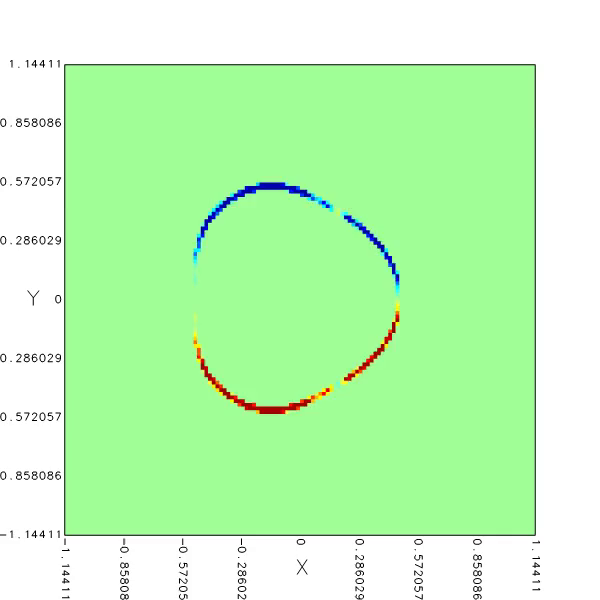
\includegraphics[width=0.23\textwidth]{image/Tension/Asym0002.png}
    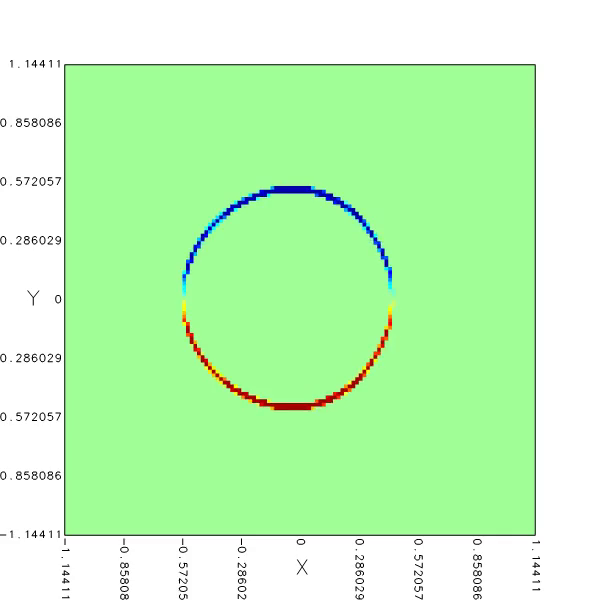
\includegraphics[width=0.23\textwidth]{image/Tension/Asym0003.png}
    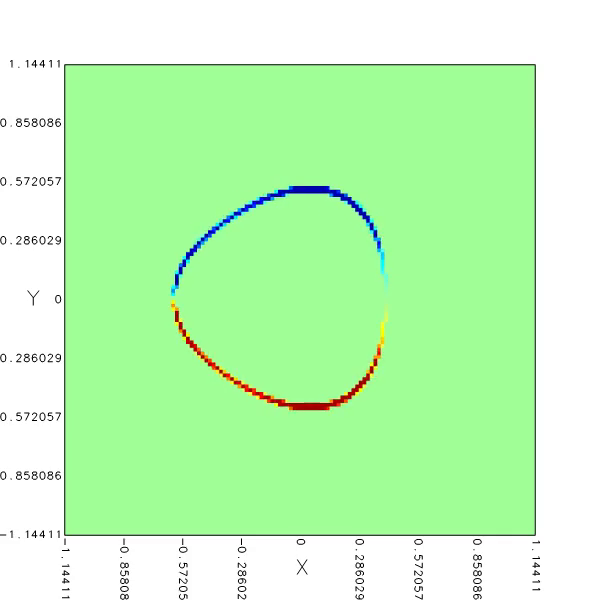
\includegraphics[width=0.23\textwidth]{image/Tension/Asym0004.png}
    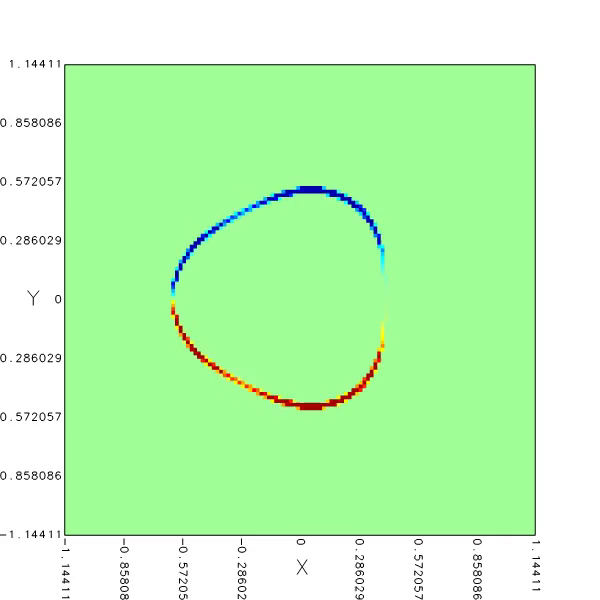
\includegraphics[width=0.23\textwidth]{image/Tension/Asym0005.png}
    % 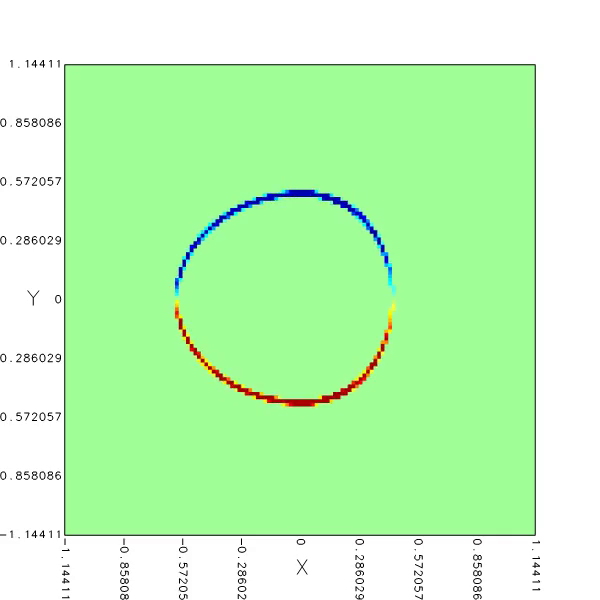
\includegraphics[width=0.2\textwidth]{image/Tension/Asym0006.png}
    \caption{Acceleration field $a_y$ for $t /T_\sigma = 1, 2, 3, 4$}
\end{figure}
\begin{figure}[h!]
    \centering
    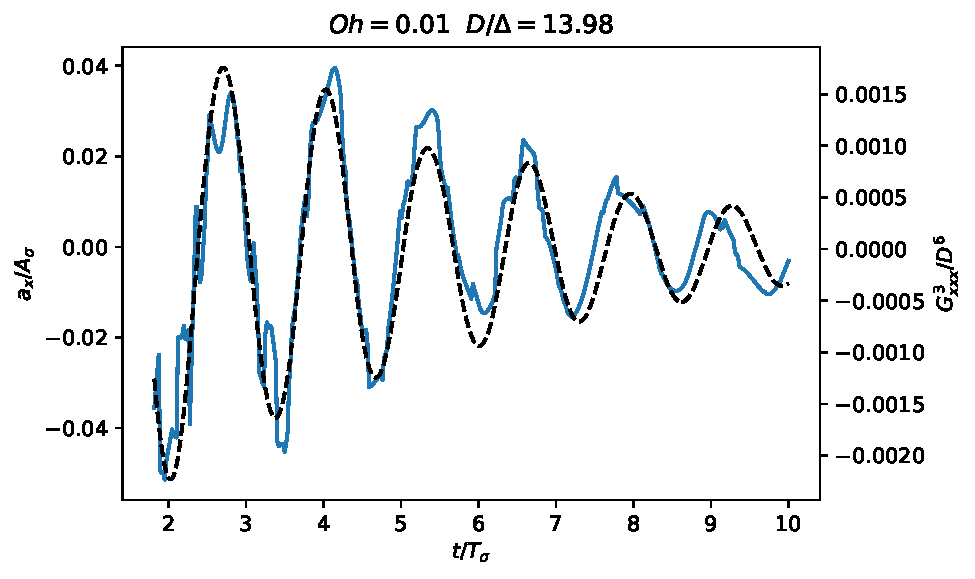
\includegraphics[width=0.4\textwidth]{image/Tension/Asym/Ax_Bo_0_1_ndc_10.pdf}
    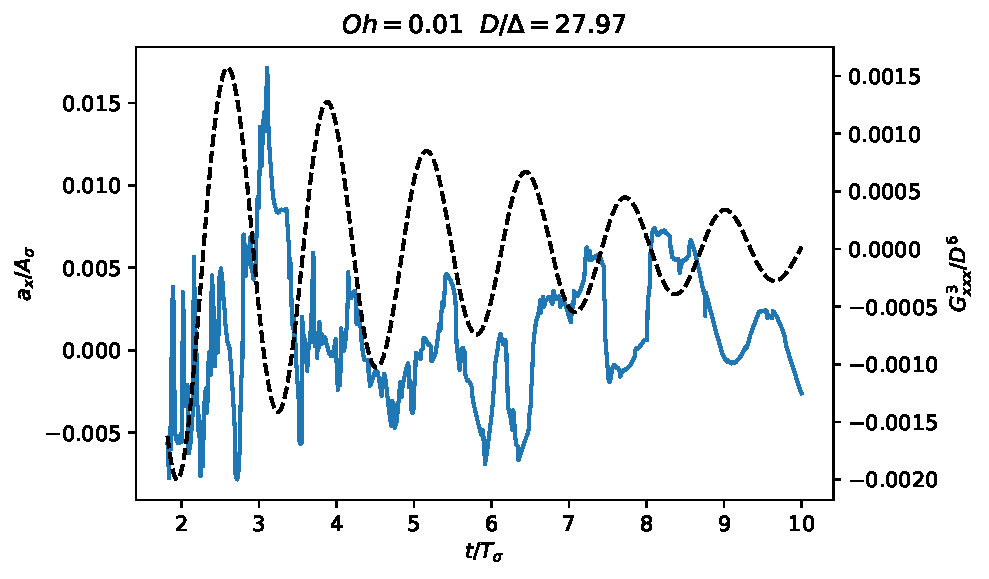
\includegraphics[width=0.4\textwidth]{image/Tension/Asym/Ax_Bo_0_1_ndc_20.pdf}
    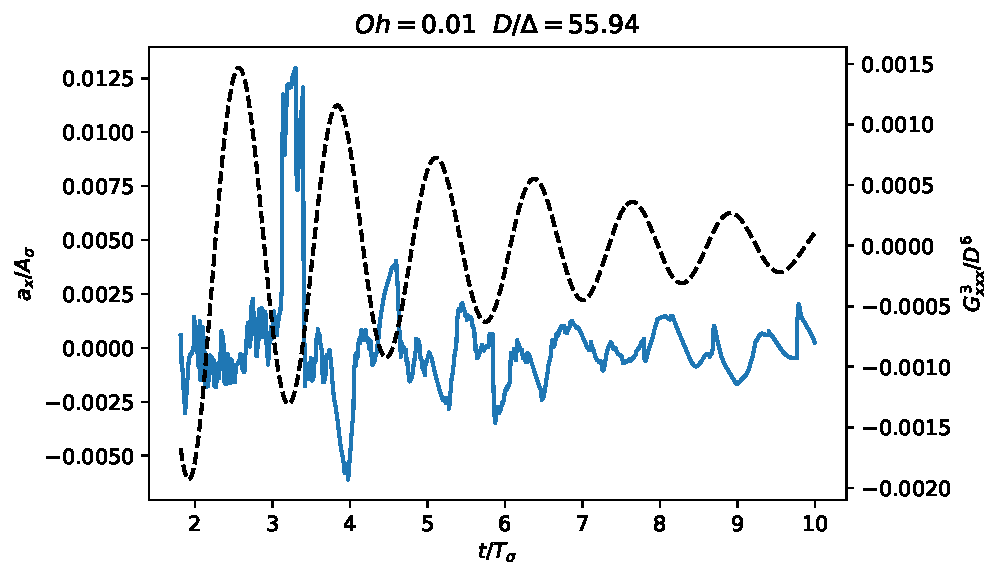
\includegraphics[width=0.4\textwidth]{image/Tension/Asym/Ax_Bo_0_1_ndc_30.pdf}
    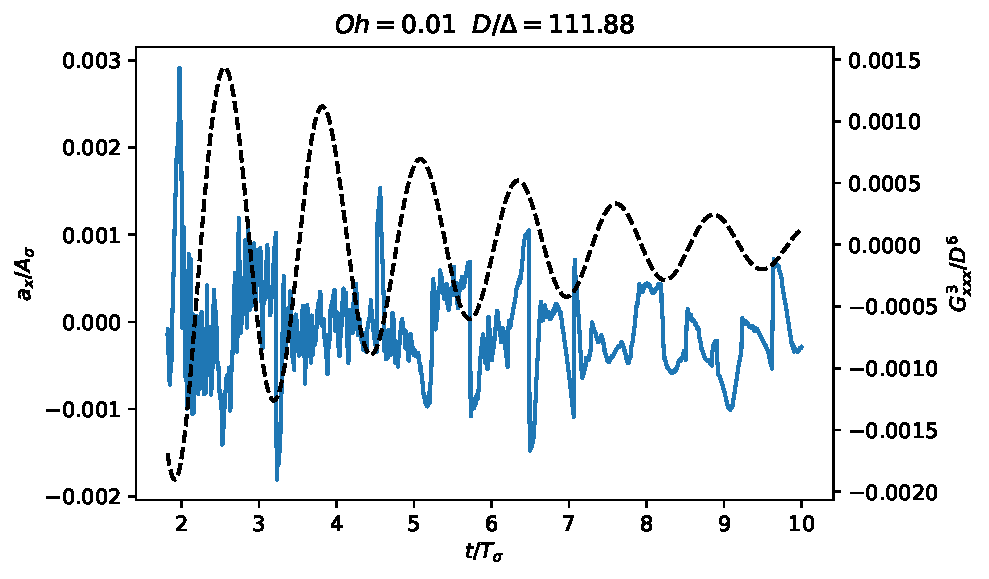
\includegraphics[width=0.4\textwidth]{image/Tension/Asym/Ax_Bo_0_1_ndc_60.pdf}
    \caption{Acceleration field $a_y$ for $t /T_\sigma = 1, 2, 3, 4$}
\end{figure}

\subsection{Moment of the surface tension on Elliptical drop}


\end{document}